\documentclass[11pt,a4paper,DIV=12]{scrartcl}

% ----------------------------------------------------------------------------
% Editable title-page fields  --  adjust the bracketed placeholders
% ----------------------------------------------------------------------------
\newcommand{\thetitle}{Classical NLP for Sentiment and Aspect-Based Analysis of Amazon Reviews}
\newcommand{\thesubtitle}{A Study of the Trade-off Between Predictive Performance and Interpretability}
\newcommand{\theauthor}{Ivelina Yaneva}
\newcommand{\thematric}{3185090}
\newcommand{\thechair}{Chair of Information Systems and Business Analytics}
\newcommand{\theseminar}{Seminar: Enterprise AI and Urban Analytics}
\newcommand{\thesupervisor}{Viet Nguyen}
\newcommand{\theplace}{W\"urzburg}

% ----------------------------------------------------------------------------
\usepackage[utf8]{inputenc}
\usepackage[T1]{fontenc}
\usepackage{mathptmx}
\usepackage[english]{babel}
\usepackage{graphicx}
\usepackage{epstopdf}          % lets Overleaf include the .eps seal directly
\usepackage{booktabs}
\usepackage{tabularx}
\usepackage{amsmath,amssymb}
\usepackage{siunitx}
\usepackage{caption}
\usepackage{subcaption}
\usepackage{float}
\usepackage{xcolor}
\usepackage[expansion=false]{microtype}
\usepackage[round]{natbib}
\usepackage{enumitem}
\usepackage[hidelinks]{hyperref}

\graphicspath{{figures/}{./}}
\definecolor{navy}{HTML}{1E3A6E}
\captionsetup{font=small,labelfont=bf}
\setlength{\parskip}{0.4em}
\sisetup{detect-weight=true,detect-family=true}

\title{\thetitle}
\author{\theauthor}

\begin{document}

% ============================ TITLE PAGE ====================================
\begin{titlepage}
\centering
{\large \theseminar \par}
\vspace{0.5cm}
{\large Seminar Paper \par}
\vspace{1.5cm}
{\Huge \bfseries \thetitle \par}
\vspace{0.6cm}
{\Large \thesubtitle \par}
\vspace{1.4cm}

\IfFileExists{uni-siegel2-eps-converted-to.pdf}
  {\includegraphics[height=6.5cm]{uni-siegel2-eps-converted-to.pdf}}
  {\IfFileExists{uni-siegel2.pdf}
    {
\includegraphics[height=6.5cm]{uni-siegel2.pdf}}
    {
\includegraphics[height=6.5cm]{uni-siegel2.eps}}}

\vspace{1.4cm}
{\large \theauthor \par}
{\normalsize Matriculation number: \thematric \par}
\vspace{0.3cm}
{\normalsize \theplace, \today \par}
\vfill
{\normalsize
Julius-Maximilians-Universit\"at W\"urzburg\\[2pt]
\thechair\\[2pt]
Supervisor: \thesupervisor\par}
\end{titlepage}

% ============================ ABSTRACT ======================================
\section*{Abstract}
\noindent
Online reviews pair a star rating with free text that explains it, offering a
continuous, survey-free feedback signal --- if the text can be read at scale.
This paper builds an end-to-end classical NLP pipeline (no large language
models) that turns 87{,}713 Amazon reviews from two subscription categories into
structured opinion data, and studies the central trade-off between predictive
performance and interpretability. For document-level polarity (RQ1) we compare a
majority-class baseline against Naive Bayes, Logistic Regression and gradient
boosting on TF-IDF features, under binary and ternary framings and with explicit
class-imbalance handling. Logistic Regression with balanced class weights is the
strongest model (binary macro-F1 $0.87$) while remaining fully interpretable;
the headline accuracy of a trivial baseline ($69\%$) is shown to be misleading
because it never identifies a single negative review. A ternary framing exposes
the hard ceiling of the task: the minority 3-star (neutral) class collapses to
$0.4\%$ recall without rebalancing. For aspect-based sentiment (RQ2) we segment
reviews into sentences, detect seven aspects with a keyword lexicon and a
noun-phrase view, and score each aspect-mentioning sentence with VADER --- a
lexicon scorer chosen because the document classifier is out-of-distribution on
single sentences. Across both categories, \emph{billing} (cancel/refund/charged)
is the clear pain point, while \emph{content} and \emph{price} are the most
positive aspects. Crucially, the strongest negative coefficient of the
interpretable classifier is the token \emph{cancel} --- the same billing signal
RQ2 surfaces independently, a convergence of two methods on one business
conclusion.

\clearpage
\tableofcontents
\clearpage

% ============================ 1 INTRODUCTION ================================
\section{Introduction}
\label{sec:intro}

Every day, millions of customers leave reviews on platforms such as Amazon,
Yelp and Google Maps. Each review couples a structured signal --- an overall
star rating --- with a block of free text explaining the reasons behind it. For
a company, this is a continuous stream of customer feedback that requires no
surveys; the difficulty is reading it at scale. \emph{Sentiment analysis}, the
task of inferring opinion polarity from text \citep{pang2008opinion}, makes this
tractable, and \emph{aspect-based sentiment analysis} (ABSA) refines it by
attributing sentiment to specific facets such as delivery, price or quality
\citep{pontiki2014semeval}.

This paper deliberately restricts itself to \emph{classical} natural language
processing and machine learning --- bag-of-words features and linear or
tree-based classifiers --- without any large language model. This is not only a
constraint but a research lens: classical models are cheap, reproducible and,
above all, \emph{interpretable}, and the central question of this work is how
much predictive performance, if any, that interpretability costs. We study two
Amazon review categories from the 2023 release \citep{hou2024bridging} and
pursue one overarching and two specific research questions.

\begin{description}[leftmargin=1.4em,style=nextline]
  \item[Main RQ] What is the trade-off between predictive performance and
  interpretability when classical machine learning is applied to review
  sentiment and product-aspect extraction?
  \item[RQ1] How accurately do classical models classify review-level
  sentiment, how does class imbalance affect their evaluation, and which review
  types are hardest to classify?
  \item[RQ2] Which product aspects do customers discuss, and how do aspect
  sentiment profiles differ between two product categories?
\end{description}

\paragraph{Contributions.}
(i)~A reproducible classical pipeline (cleaning, TF-IDF features, three
classifier families, evaluation) with an honest treatment of class imbalance,
showing that accuracy is the wrong headline metric and that a balanced Logistic
Regression matches gradient boosting while staying interpretable.
(ii)~An unsupervised, sentence-level ABSA pipeline using a domain-adapted aspect
lexicon and VADER, with a robustness check against the document classifier.
(iii)~A cross-method finding: the most negative linear-model coefficient and the
most negative VADER aspect independently identify \emph{billing} as the dominant
source of dissatisfaction for subscription products.

% ============================ 2 RELATED WORK ================================
\section{Background and Related Work}
\label{sec:related}

\subsection{Sentiment analysis}
Opinion mining and sentiment analysis are surveyed comprehensively by
\citet{pang2008opinion}, who frame polarity classification as a supervised
learning problem over textual features and discuss the role of domain, negation
and subjectivity. A long line of work treats document-level polarity as text
classification with bag-of-words or n-gram features
\citep{maas2011learning,manning2008introduction}; we follow this classical
recipe rather than dense neural representations.

\subsection{Aspect-based sentiment analysis}
\citet{pontiki2014semeval} formalise ABSA in SemEval-2014 Task~4, distinguishing
aspect-term extraction, aspect-category detection and per-aspect polarity, and
provide gold-annotated benchmarks. Their setting is supervised; in the absence of
aspect-level annotations for the Amazon categories studied here, we approximate
the same goals with an unsupervised lexicon-plus-VADER approach (Section
\ref{sec:method-rq2}), which trades annotation cost for transparency.

\subsection{Features, models and lexicon scoring}
TF-IDF weighting over unigrams and bigrams is the standard sparse text
representation \citep{manning2008introduction}. We compare three classifier
families that span the bias--variance and interpretability spectrum: Multinomial
Naive Bayes (a generative linear baseline), Logistic Regression (a discriminative
linear model whose weights are directly readable), and gradient-boosted decision
trees via LightGBM \citep{ke2017lightgbm}. For sentence-level sentiment we use
VADER \citep{hutto2014vader}, a rule-based valence lexicon designed for short,
informal text that needs no training data. All models are implemented with
scikit-learn \citep{pedregosa2011scikit}, spaCy \citep{honnibal2017spacy} and
NLTK \citep{bird2009natural}.

\subsection{Why classical, and the neural contrast}
Transformer sentence encoders such as Sentence-BERT \citep{reimers2019sentencebert}
achieve strong results on semantic tasks but are comparatively opaque and
resource-intensive. For an operational feedback dashboard, the value of a model
that can answer ``\emph{which words drove this prediction?}'' is high. Our study
therefore quantifies what is given up by staying classical, and finds (Section
\ref{sec:discussion}) that on these high-dimensional sparse features the
interpretable linear model is not outperformed by the more complex tree ensemble.

% ============================ 3 DATA & EDA ==================================
\section{Dataset and Exploratory Analysis}
\label{sec:eda}

\subsection{Dataset and category choice}
We use the Amazon Reviews 2023 dataset \citep{hou2024bridging}. The task asks for
the smallest category; because RQ2 requires a \emph{cross-category} comparison,
we deliberately analyse \emph{two} categories: \textbf{Subscription Boxes}
(16{,}216 reviews, 641 distinct items --- among the smallest categories) and
\textbf{Magazine Subscriptions} (71{,}497 reviews), for a combined
\textbf{87{,}713} reviews. Each review provides a 1--5 star \texttt{rating}, a
\texttt{title}, free-text \texttt{body}, a \texttt{timestamp}, a
\texttt{verified\_purchase} flag and a \texttt{helpful\_vote} count. Table
\ref{tab:eda} summarises the key statistics.

\begin{table}[H]
\centering
\caption{Key dataset statistics from the exploratory analysis.}
\label{tab:eda}
\begin{tabular}{lr}
\toprule
Statistic & Value \\
\midrule
Total reviews & 87{,}713 \\
\quad Subscription Boxes & 16{,}216 \\
\quad Magazine Subscriptions & 71{,}497 \\
Time span & 2001--2023 \\
Verified-purchase share & 82.7\,\% \\
Mean / median review length & 40 / 22 words \\
5-star share & 60.8\,\% \\
1-star share & 14.0\,\% \\
Binary imbalance (pos:neg) & 3.57 : 1 \\
Neutral (3-star) share & 7.7\,\% \\
Vocabulary size (\(\mathrm{min\_df}=5\)) & 6{,}308 \\
\bottomrule
\end{tabular}
\end{table}

\subsection{Star distribution and class imbalance}
The rating distribution is strongly positive-skewed: $60.8\%$ of reviews are
5-star and only $14.0\%$ are 1-star (Figure \ref{fig:stars}). Mapping ratings to
sentiment (Section \ref{sec:method-label}) yields a $3.57\!:\!1$
positive-to-negative imbalance in the binary framing and a small $7.7\%$ neutral
class in the ternary framing (Figure \ref{fig:imbalance}). This imbalance is the
single most important property for evaluation: a classifier that always predicts
``positive'' already attains high accuracy while being useless, which is why we
report macro-F1 and per-class recall throughout.

\begin{figure}[H]
\centering
\begin{subfigure}{0.49\textwidth}
  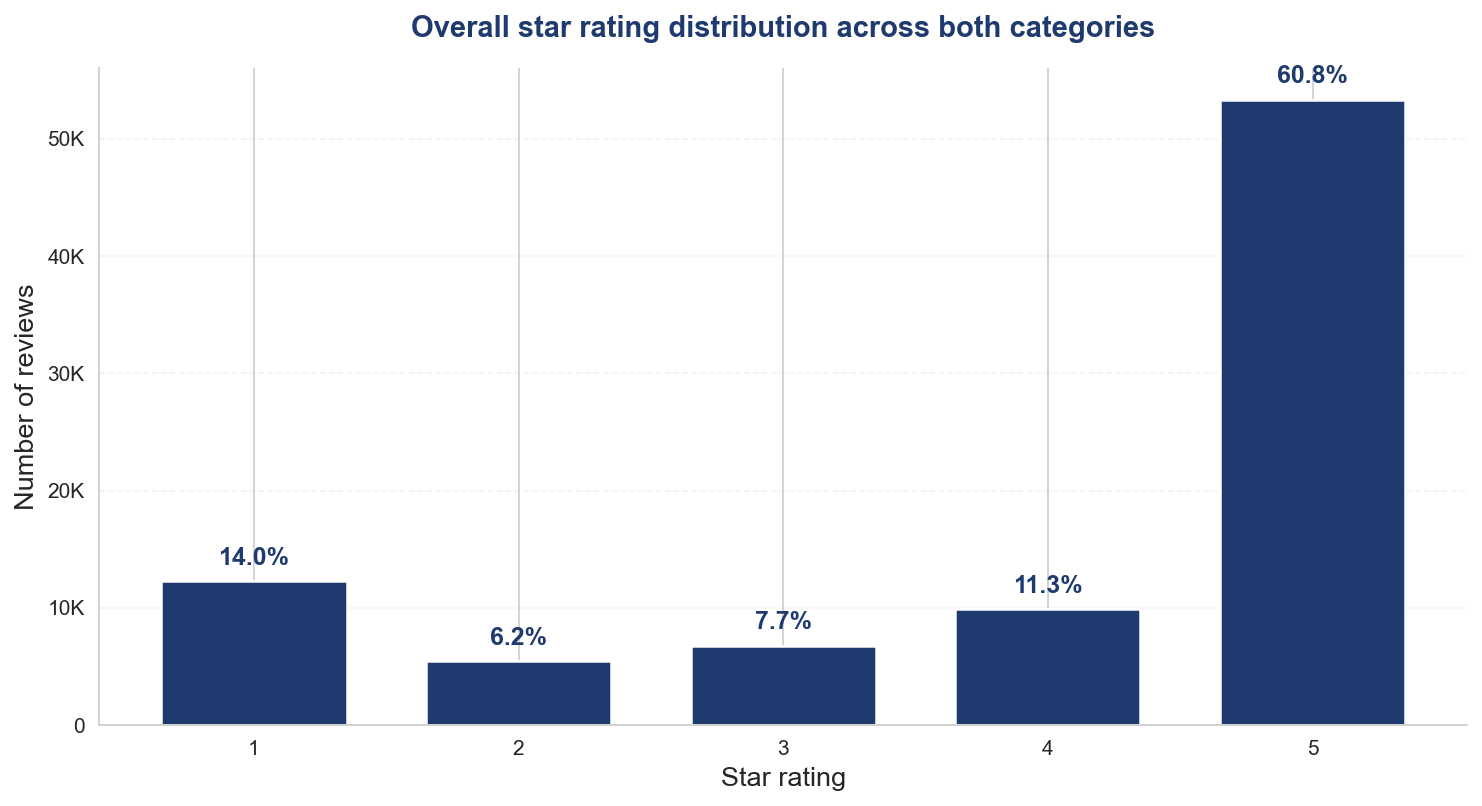
\includegraphics[width=\linewidth]{star_distribution_overall.png}
  \caption{Overall star distribution.}
\end{subfigure}\hfill
\begin{subfigure}{0.49\textwidth}
  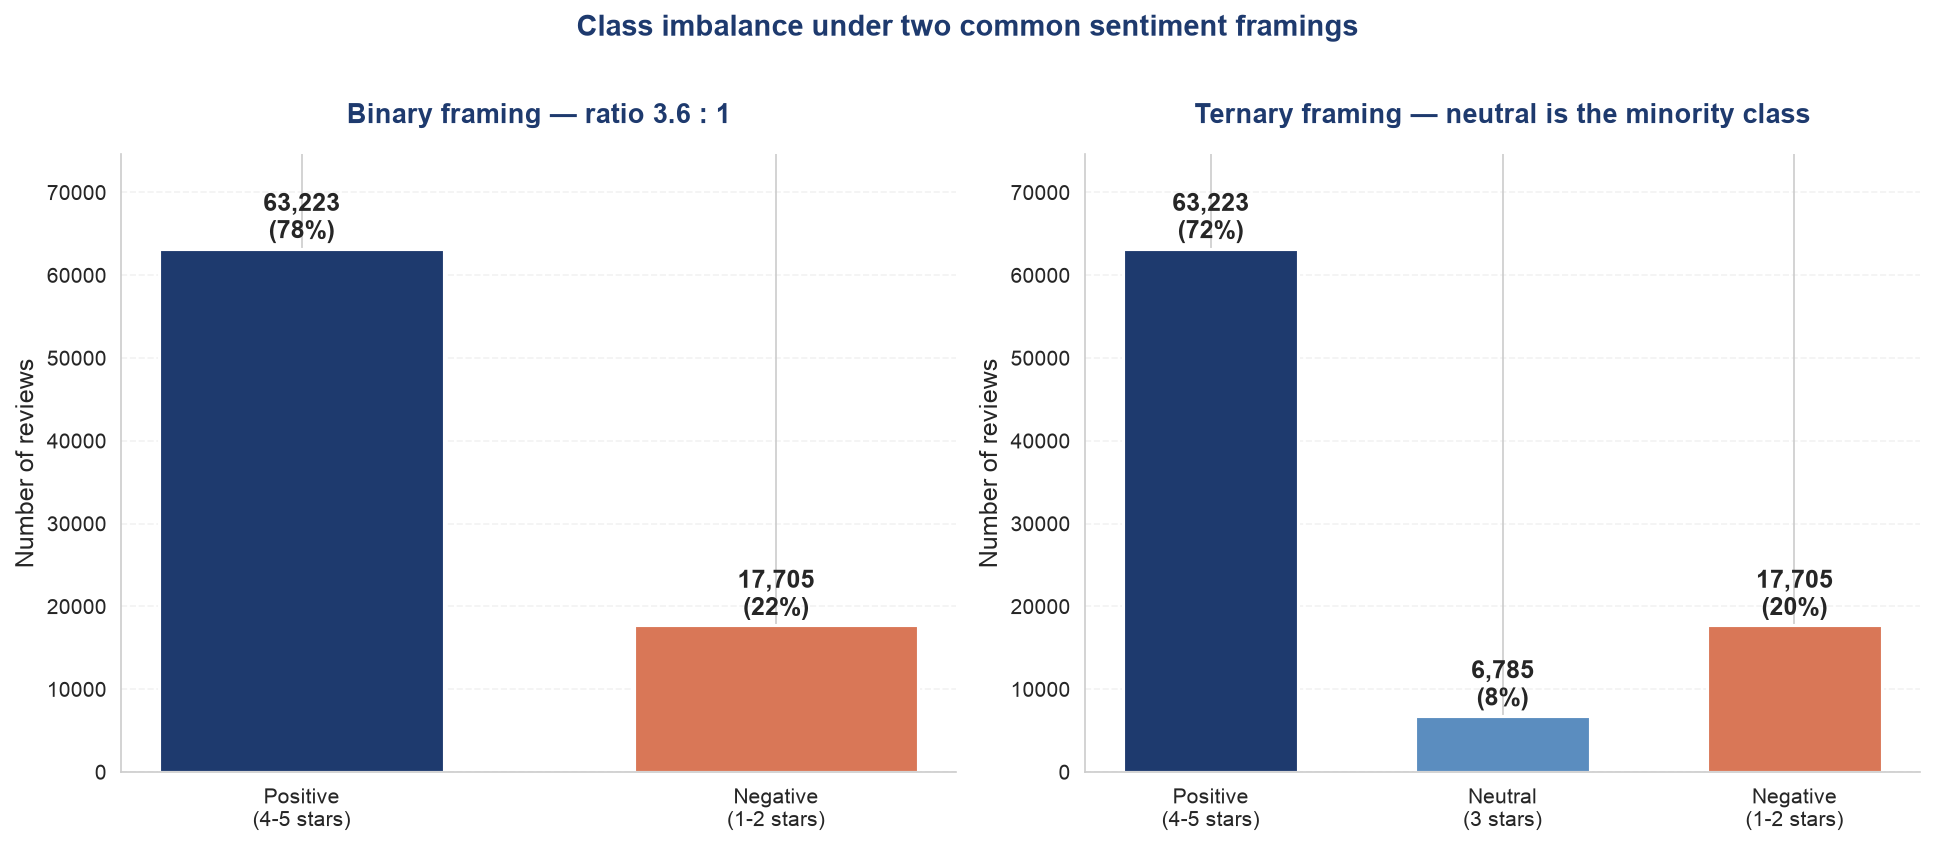
\includegraphics[width=\linewidth]{class_imbalance.png}
  \caption{Sentiment-class imbalance.}
\end{subfigure}
\caption{Star ratings are heavily skewed toward 5 stars, producing a substantial
positive/negative imbalance and a small neutral class.}
\label{fig:stars}
\end{figure}

\begin{figure}[H]
\centering
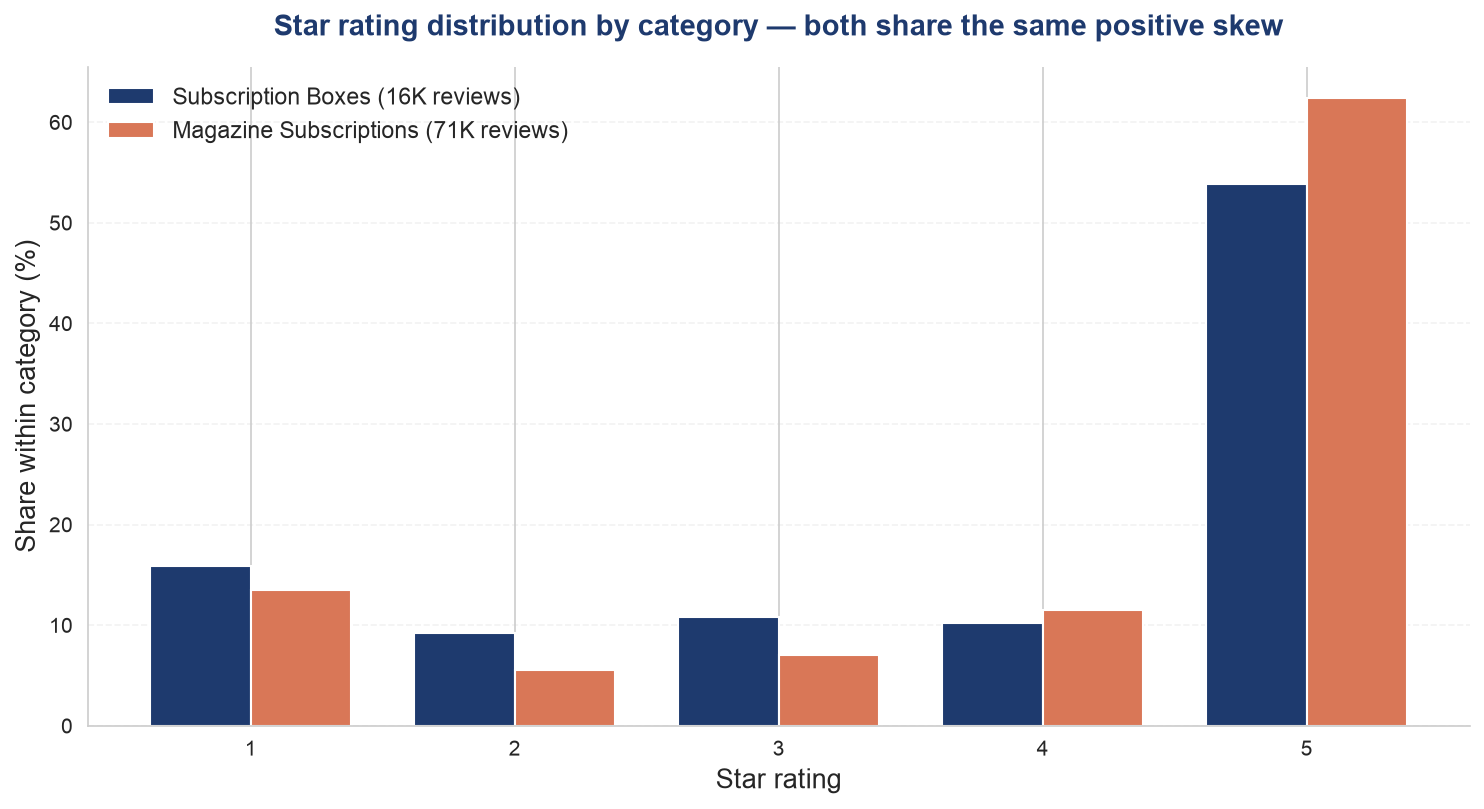
\includegraphics[width=0.62\textwidth]{star_distribution_by_category.png}
\caption{Per-category star distribution: both categories share the positive
skew, confirming the imbalance is not an artefact of one category.}
\label{fig:imbalance}
\end{figure}

\subsection{Review length and vocabulary}
Reviews are short: a median of 22 words and a mean of 40 (Figure
\ref{fig:length}). Short texts carry few features, which both favours sparse
linear models and motivates the sentence-level treatment in RQ2. A
whitespace-tokenised vocabulary on a 20K-review sample, filtered at
$\mathrm{min\_df}=5$, contains roughly $6{,}300$ terms.

\begin{figure}[H]
\centering
\begin{subfigure}{0.49\textwidth}
  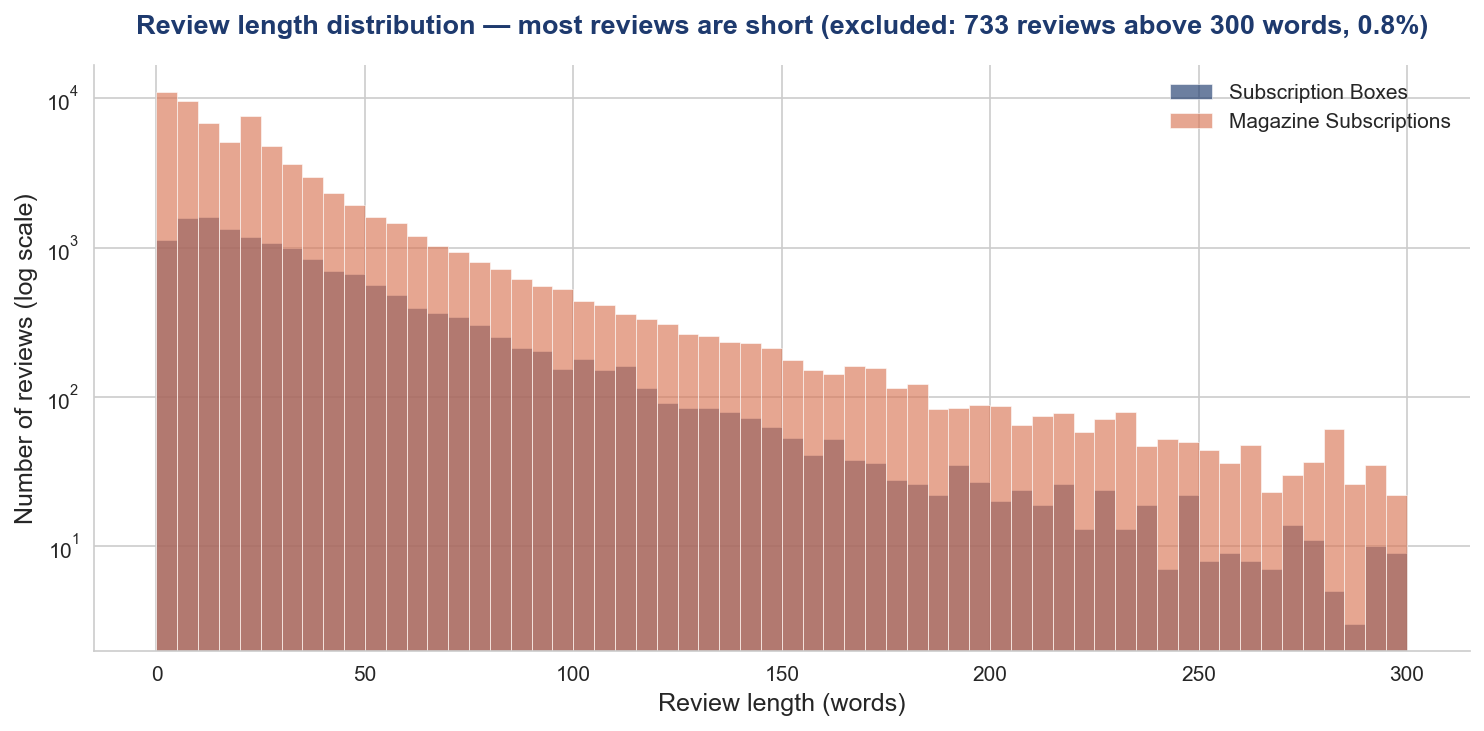
\includegraphics[width=\linewidth]{review_length_histogram.png}
  \caption{Review-length distribution (words).}
\end{subfigure}\hfill
\begin{subfigure}{0.49\textwidth}
  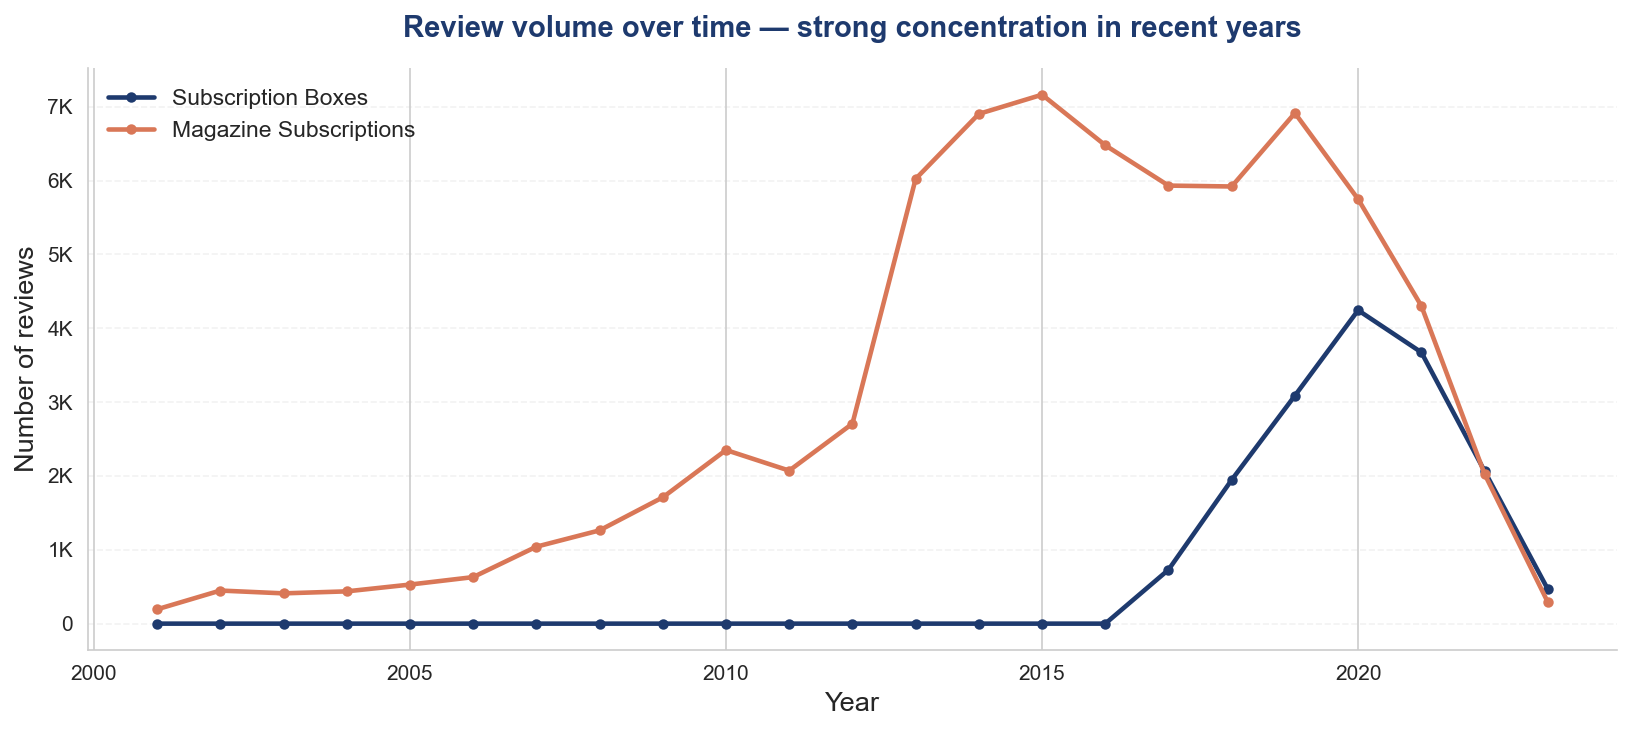
\includegraphics[width=\linewidth]{reviews_over_time.png}
  \caption{Review volume over time.}
\end{subfigure}
\caption{Most reviews are short, and review volume is concentrated in recent
years --- which motivates a chronological rather than random train/test split.}
\label{fig:length}
\end{figure}

\subsection{Discriminative terms}
A weighted log-odds analysis with an informative Dirichlet prior
\citep{monroe2008fightin} identifies the terms most associated with each
sentiment class. Rendered as word clouds (Figure \ref{fig:wordcloud}), the
positive class is dominated by generic affect (\emph{love, great, enjoy,
wonderful}), while the negative class is strikingly concrete: \emph{cancel,
refund, subscription, ad, advertisement, charge, renewal}. Already at the
descriptive stage, the data points to billing and advertising as the negative
themes that the modelling later confirms.

\begin{figure}[H]
\centering
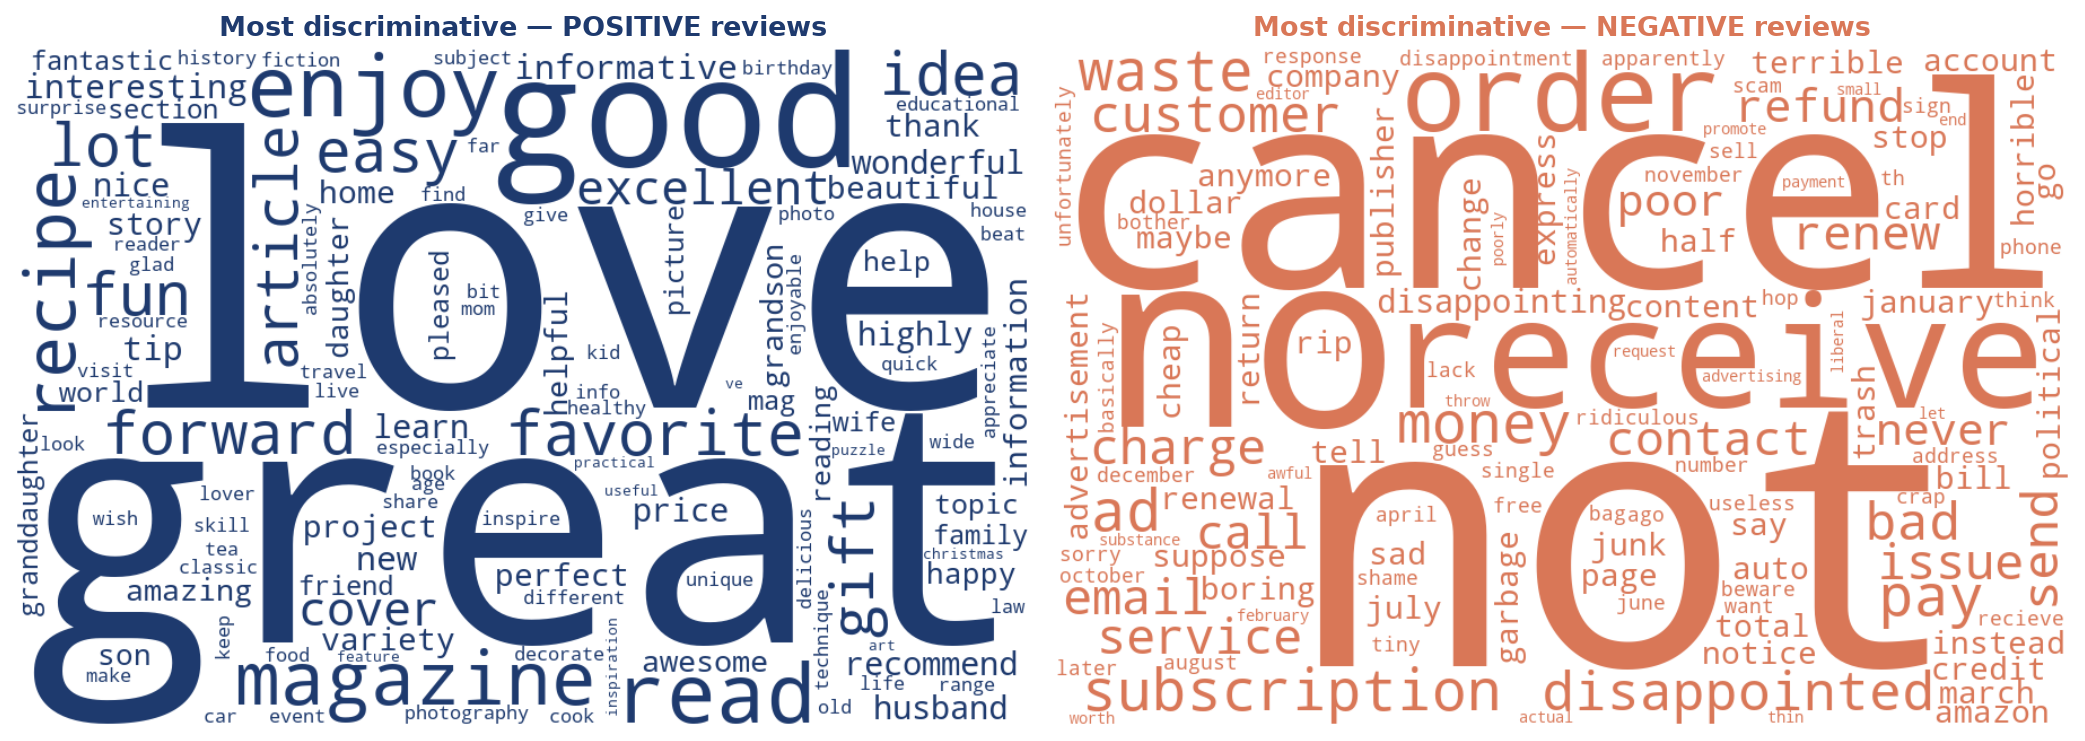
\includegraphics[width=\textwidth]{wordcloud_sentiment.png}
\caption{Most discriminative terms per sentiment class (size $\propto$ weighted
log-odds z-score). The negative cloud is a billing/advertising cluster.}
\label{fig:wordcloud}
\end{figure}

% ============================ 4 METHOD ======================================
\section{Methodology}
\label{sec:method}

\subsection{Sentiment labelling}
\label{sec:method-label}
Star ratings are the natural supervision signal but exist only per review, so
RQ1 operates at the document level. We use two framings. The \textbf{binary}
framing maps 1--2 stars to \emph{negative}, 4--5 to \emph{positive} and drops
3-star reviews; the \textbf{ternary} framing keeps 3 stars as \emph{neutral}.
Binary leads the analysis; ternary is reported to probe the hard, mixed-sentiment
middle.

\subsection{Text preprocessing}
The body text is lowercased and stripped of HTML, URLs and non-alphabetic
characters, then tokenised, stopword-filtered and lemmatised with spaCy
(\texttt{en\_core\_web\_sm}). A small number of reviews ($275$) reduce to an
empty string and are dropped before modelling, as they carry no bag-of-words
signal. The cleaned text feeds only the TF-IDF classifiers of RQ1; VADER in RQ2
deliberately consumes the \emph{raw} text, because its valence rules exploit
capitalisation, punctuation and intensifiers.

\subsection{Chronological train/test split}
Because review volume is concentrated in recent years, a random split would let a
model train on future reviews. We therefore sort by timestamp and use the oldest
$80\%$ for training and the newest $20\%$ for testing, performed \emph{within each
category} so that both categories appear on both sides --- preserving the
cross-category comparison RQ2 needs while making evaluation mimic deployment.

\subsection{Features}
We build TF-IDF vectors with sublinear term-frequency scaling, $\mathrm{min\_df}=5$
and a vocabulary cap of $20{,}000$. Two configurations are compared: unigrams,
and unigrams+bigrams; the vectoriser is fit on the training split only.

\subsection{Models and imbalance handling}
We evaluate a \textbf{majority-class baseline} (always predicts positive),
\textbf{Multinomial Naive Bayes}, \textbf{Logistic Regression} and
\textbf{LightGBM} gradient boosting \citep{ke2017lightgbm}. Imbalance is handled
two ways: Logistic Regression and LightGBM use \texttt{class\_weight=balanced};
Naive Bayes, which has no class-weight parameter, is trained on a randomly
undersampled balanced set. Each model is run with and without handling so the
effect is visible.

\subsection{Evaluation}
We report accuracy (for reference), macro-averaged F1, weighted F1 and per-class
recall, plus confusion matrices. Macro-F1 and minority-class recall are the
primary metrics under imbalance. Error analysis ranks the most confidently wrong
predictions to characterise the hardest reviews.

\subsection{Aspect-based pipeline (RQ2)}
\label{sec:method-rq2}
A review-level label cannot express that one review praises content but
criticises price, so RQ2 works below the review. Each review is split into
sentences; aspects are detected per sentence using a curated keyword lexicon of
seven aspects --- \emph{delivery, packaging, quality, price, content, customer
service} and \emph{billing} --- the last two added because the EDA surfaced
content and billing/renewal vocabulary prominently. A complementary, lexicon-free
noun-phrase view (spaCy noun chunks) provides data-driven aspect candidates.
Each aspect-mentioning sentence is scored with VADER \citep{hutto2014vader}, and
scores are aggregated per review, per aspect and per category.

\paragraph{Why VADER rather than the RQ1 classifier.}
The RQ1 classifier is trained on whole reviews; applying it to single sentences
is an out-of-distribution use, since sentences are far shorter with a different
feature distribution. VADER needs no training and is built for short text, so it
is the \emph{primary} sentence-level scorer. The document classifier is retained
only as a \emph{robustness check}: we measure how often the two methods agree
rather than assuming either is ground truth (Section \ref{sec:rq2-robust}).

% ============================ 5 RESULTS RQ1 =================================
\section{Results: Document-Level Sentiment (RQ1)}
\label{sec:rq1}

\subsection{Binary framing}
Table \ref{tab:rq1bin} reports the binary results on the held-out test set. The
majority baseline reaches $68.9\%$ accuracy but macro-F1 $0.408$ and
\textbf{zero} recall on the negative class --- a vivid demonstration that
accuracy hides total minority failure. Without imbalance handling, the three
models inherit a milder version of this skew (Naive Bayes recovers only $55\%$ of
negatives). Switching on balanced weighting or undersampling lifts negative
recall to $0.87$--$0.89$. \textbf{Logistic Regression with balanced weights is
the best overall model} (accuracy $0.885$, macro-F1 $0.870$, both classes
recalled near $0.88$); here, balancing even \emph{improves} accuracy because the
unbalanced model was sacrificing too many negatives. Figures
\ref{fig:rq1conf} and \ref{fig:rq1bars} visualise the recovery.

\begin{table}[H]
\centering
\caption{RQ1 binary model comparison (test set). Macro-F1 and per-class recall
are primary; accuracy is reference only. Best macro-F1 in \textbf{bold}.}
\label{tab:rq1bin}
\begin{tabular}{lrrrr}
\toprule
Model & Accuracy & Macro-F1 & Recall$_{\text{pos}}$ & Recall$_{\text{neg}}$ \\
\midrule
Majority baseline            & 0.689 & 0.408 & 1.000 & 0.000 \\
Naive Bayes                  & 0.840 & 0.787 & 0.971 & 0.550 \\
Logistic Regression          & 0.871 & 0.838 & 0.961 & 0.672 \\
Gradient Boosting            & 0.857 & 0.817 & 0.961 & 0.628 \\
Naive Bayes (resampled)      & 0.860 & 0.845 & 0.844 & 0.894 \\
\textbf{Logistic Reg.\ (balanced)} & \textbf{0.885} & \textbf{0.870} & 0.889 & 0.875 \\
Gradient Boosting (balanced) & 0.850 & 0.834 & 0.843 & 0.867 \\
\bottomrule
\end{tabular}
\end{table}

\begin{figure}[H]
\centering
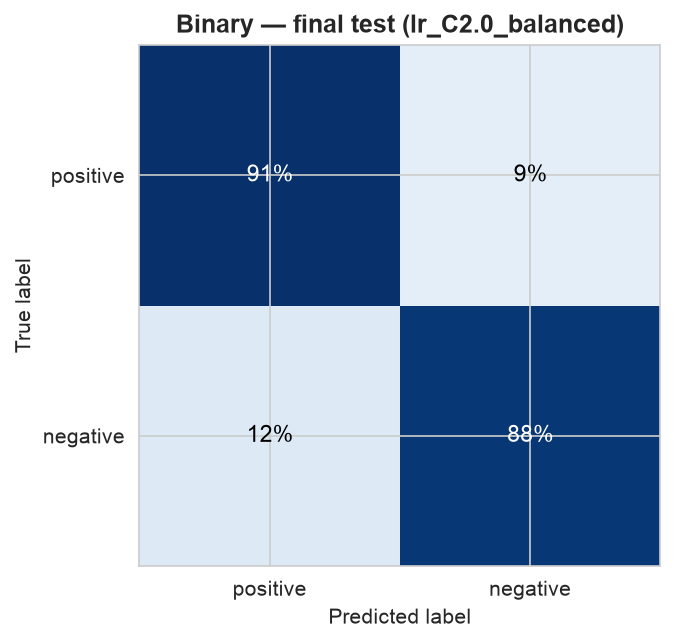
\includegraphics[width=\textwidth]{rq1_confusion_binary.png}
\caption{Binary confusion matrices (row-normalised). Balanced class weighting
turns a model that misses a third of negatives into one that recalls them
evenly.}
\label{fig:rq1conf}
\end{figure}

\begin{figure}[H]
\centering
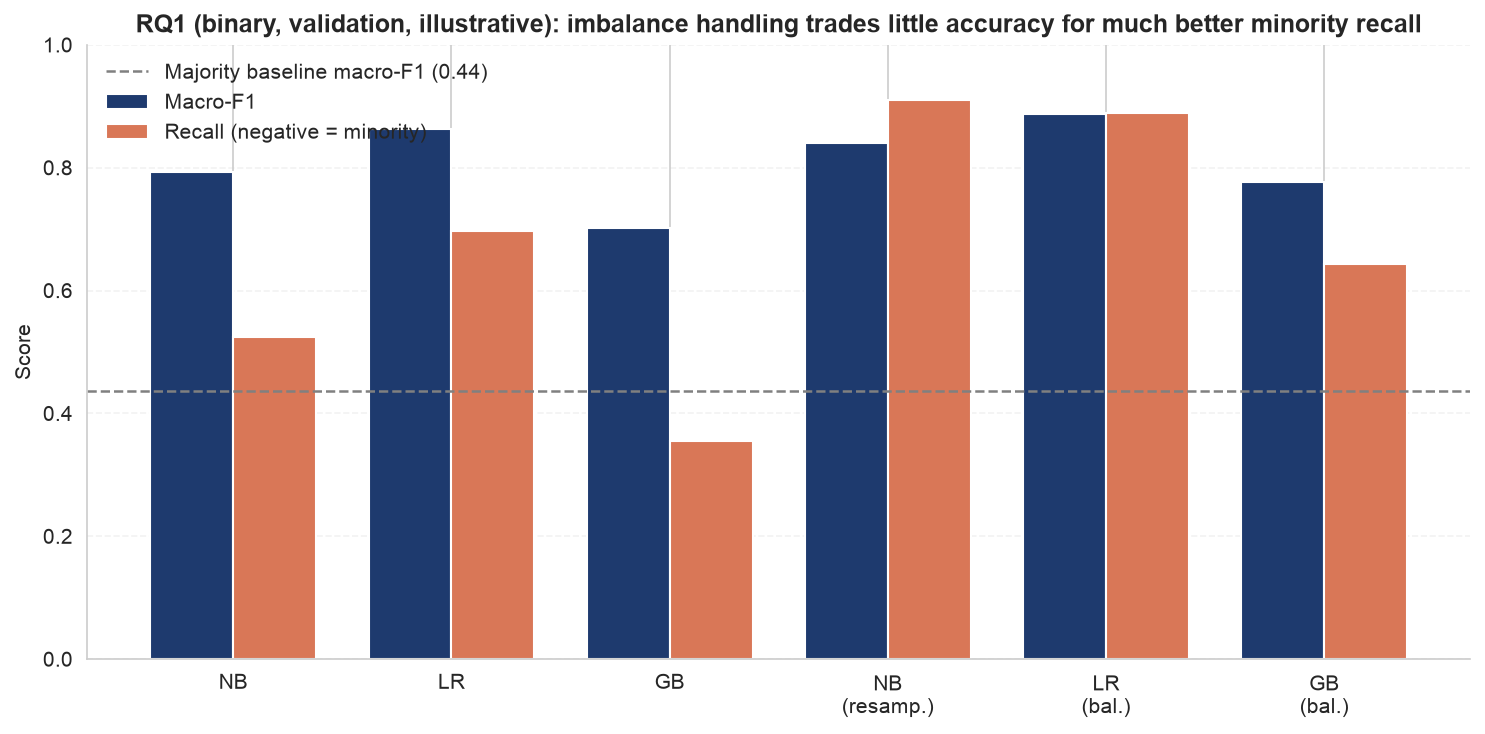
\includegraphics[width=0.92\textwidth]{rq1_imbalance_comparison.png}
\caption{Macro-F1 and minority-class (negative) recall, with and without
imbalance handling. The dashed line is the majority-baseline macro-F1.}
\label{fig:rq1bars}
\end{figure}

\subsection{Ternary framing}
Adding the 3-star neutral class makes the task markedly harder (Table
\ref{tab:rq1tern}). Without handling, Naive Bayes predicts the neutral class with
$0.4\%$ recall --- a textbook minority collapse --- and even Logistic Regression
reaches only $9\%$. Balancing raises Logistic Regression's neutral recall to
$42\%$ and Naive Bayes' (resampled) to $50\%$, but at a genuine accuracy cost
($0.81 \rightarrow 0.77$ for LR). This is the central RQ1 trade-off: the 3-star
class never becomes easy because such reviews genuinely mix positive and negative
content, which directly motivates the sentence-level view of RQ2.

\begin{table}[H]
\centering
\caption{RQ1 ternary model comparison (test set). The neutral (3-star) recall
column shows the minority collapse and its partial recovery.}
\label{tab:rq1tern}
\begin{tabular}{lrrrrr}
\toprule
Model & Acc. & Macro-F1 & Rec$_{\text{pos}}$ & Rec$_{\text{neu}}$ & Rec$_{\text{neg}}$ \\
\midrule
Majority baseline            & 0.639 & 0.260 & 1.000 & 0.000 & 0.000 \\
Naive Bayes                  & 0.780 & 0.508 & 0.970 & 0.004 & 0.551 \\
Logistic Regression          & 0.813 & 0.587 & 0.954 & 0.087 & 0.681 \\
Gradient Boosting            & 0.799 & 0.571 & 0.957 & 0.083 & 0.626 \\
Naive Bayes (resampled)      & 0.714 & 0.596 & 0.742 & 0.499 & 0.703 \\
\textbf{Logistic Reg.\ (balanced)} & 0.767 & \textbf{0.625} & 0.832 & 0.423 & 0.708 \\
Gradient Boosting (balanced) & 0.733 & 0.603 & 0.782 & 0.449 & 0.695 \\
\bottomrule
\end{tabular}
\end{table}

\begin{figure}[H]
\centering
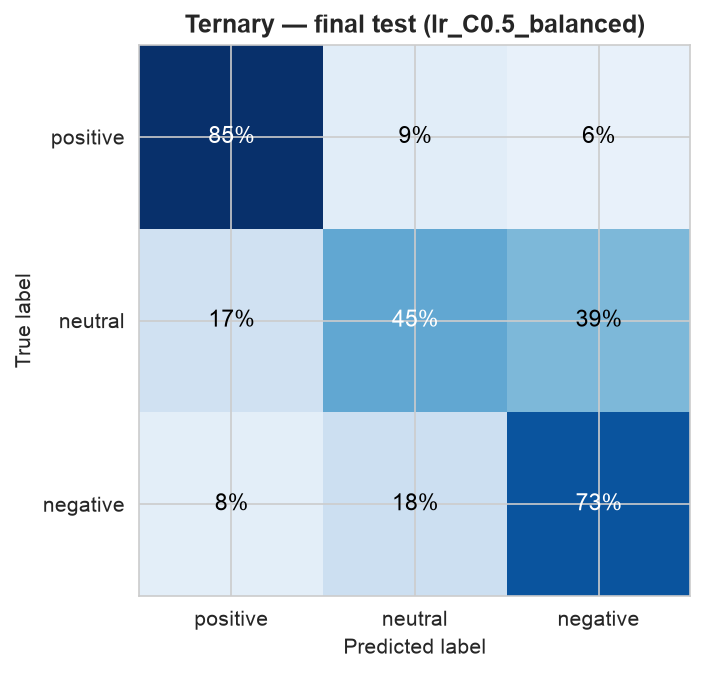
\includegraphics[width=0.5\textwidth]{rq1_confusion_ternary.png}
\caption{Ternary confusion matrix (Logistic Regression, balanced). Neutral
reviews are most often confused with the adjacent positive class.}
\label{fig:rq1ternconf}
\end{figure}

\subsection{Feature representation}
Adding bigrams roughly doubles the vocabulary ($8{,}838 \rightarrow 20{,}000$
features) for a small but real gain in macro-F1 ($0.861 \rightarrow 0.870$;
Table \ref{tab:feat}). Bigrams capture negations and short phrases (``not
worth'', ``highly recommend'') that unigrams miss. For a strictly leaner,
interpretability-first setup, unigrams remain defensible.

\begin{table}[H]
\centering
\caption{Feature comparison (Logistic Regression, balanced, binary).}
\label{tab:feat}
\begin{tabular}{lrrr}
\toprule
Features & \#\,Features & Accuracy & Macro-F1 \\
\midrule
TF-IDF unigram        & 8{,}838  & 0.876 & 0.861 \\
TF-IDF uni+bigram     & 20{,}000 & 0.885 & 0.870 \\
\bottomrule
\end{tabular}
\end{table}

\subsection{Interpretability}
A linear TF-IDF model exposes a signed weight per feature. Table \ref{tab:coef}
and Figure \ref{fig:coef} list the strongest. The positive weights are generic
affect; the negative weights are dominated by \emph{disappointed, cancel,
disappointing, ad, advertisement} and the bigram \emph{cancel subscription}.
That the single strongest negative driver is a \emph{billing} word, not a
product-quality word, is the key qualitative result of RQ1 --- and it directly
anticipates RQ2.

\begin{table}[H]
\centering
\caption{Strongest Logistic-Regression coefficients (binary, balanced).}
\label{tab:coef}
\begin{tabular}{lr@{\qquad}lr}
\toprule
Positive term & Weight & Negative term & Weight \\
\midrule
love      & $+14.6$ & disappointed        & $-7.9$ \\
great     & $+9.0$  & cancel              & $-7.7$ \\
enjoy     & $+8.0$  & disappointing       & $-6.3$ \\
excellent & $+6.4$  & ad                  & $-5.6$ \\
perfect   & $+5.7$  & poor                & $-5.5$ \\
amazing   & $+5.5$  & boring              & $-5.2$ \\
easy      & $+5.4$  & waste               & $-5.0$ \\
favorite  & $+5.3$  & advertisement       & $-4.8$ \\
\bottomrule
\end{tabular}
\end{table}

\begin{figure}[H]
\centering
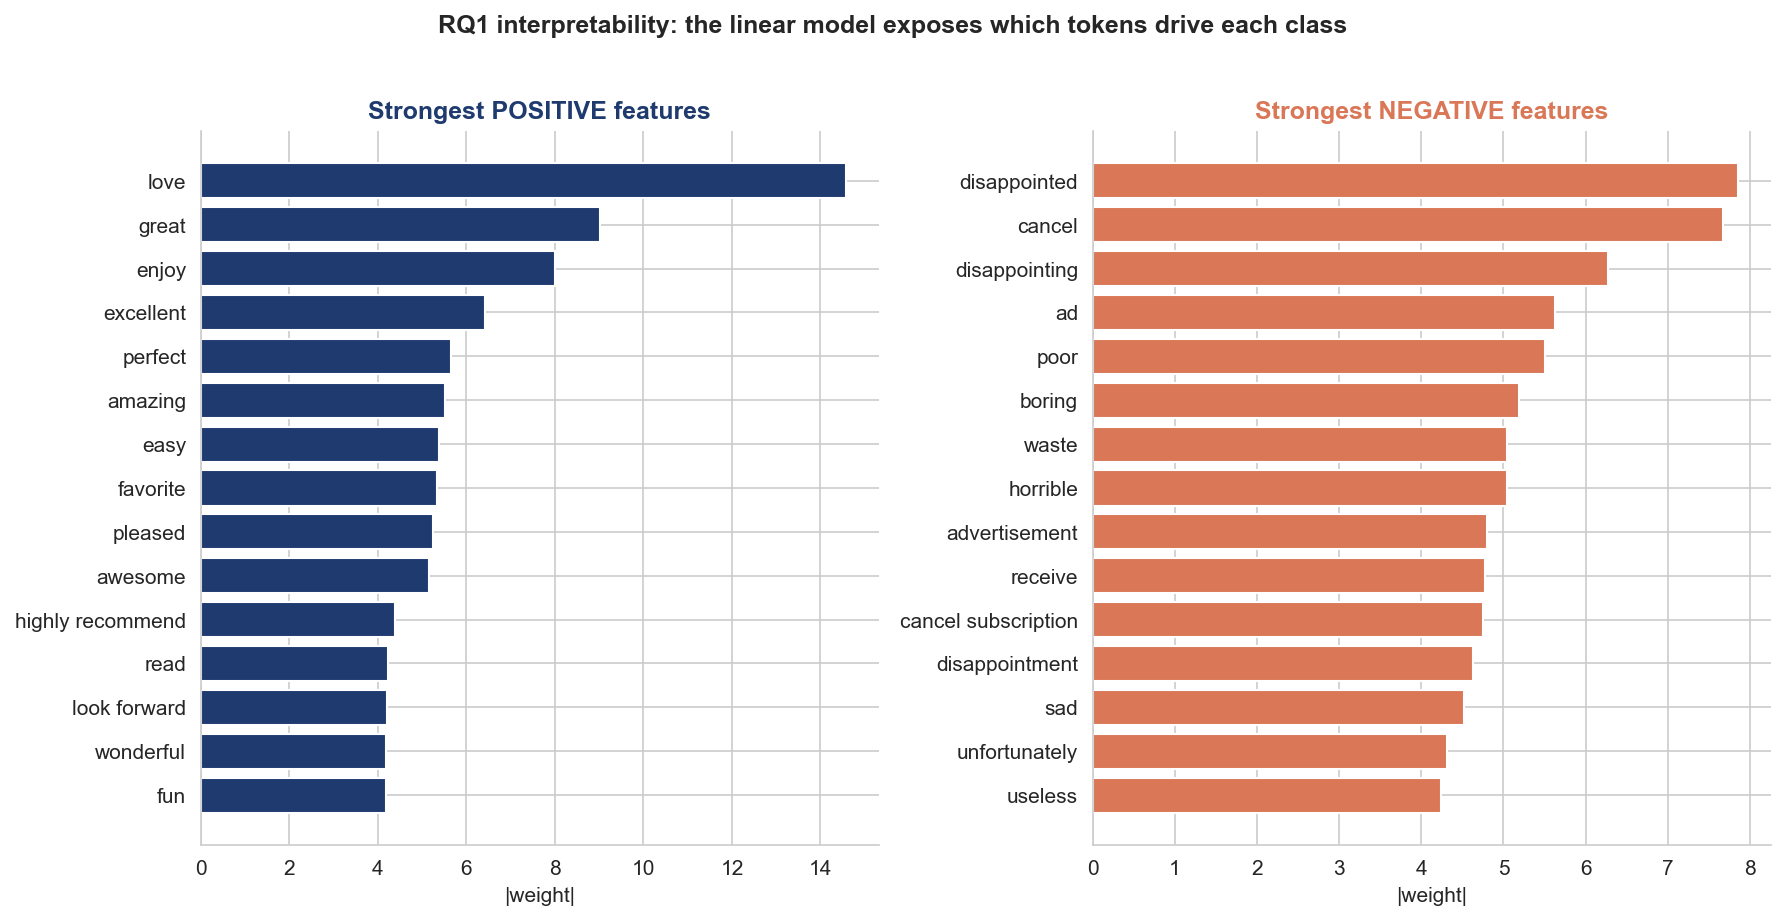
\includegraphics[width=\textwidth]{rq1_lr_coefficients.png}
\caption{The linear model is fully auditable: each token carries an explicit,
signed contribution to the positive/negative decision.}
\label{fig:coef}
\end{figure}

\subsection{Error analysis: the hardest reviews}
Ranking the most confidently wrong predictions reveals that many are not model
failures but \emph{label noise}: reviews whose star rating disagrees with their
text. Examples include 5-star reviews reading ``\emph{Very disappointed \dots
Cancelled}'', ``\emph{ad after ad \dots overpriced}'' and ``\emph{Waste of
money}'', and a 1-star review reading simply ``\emph{Perfect}''. The model's
text-based judgement is arguably correct in these cases; the star rating is the
unreliable signal. This both bounds achievable accuracy and reinforces the value
of reading the text rather than trusting the star alone.

% ============================ 6 RESULTS RQ2 =================================
\section{Results: Aspect-Based Sentiment (RQ2)}
\label{sec:rq2}

\subsection{What customers discuss}
Aspect mention rates differ sharply by category (Figure \ref{fig:rq2mention},
Table \ref{tab:rq2}). \emph{Content} dominates Magazine reviews ($63.5\%$ mention
it), whereas \emph{packaging} dominates Subscription-Box reviews ($46.5\%$): the
physical unboxing matters for boxes, the editorial substance for magazines.

\begin{figure}[H]
\centering
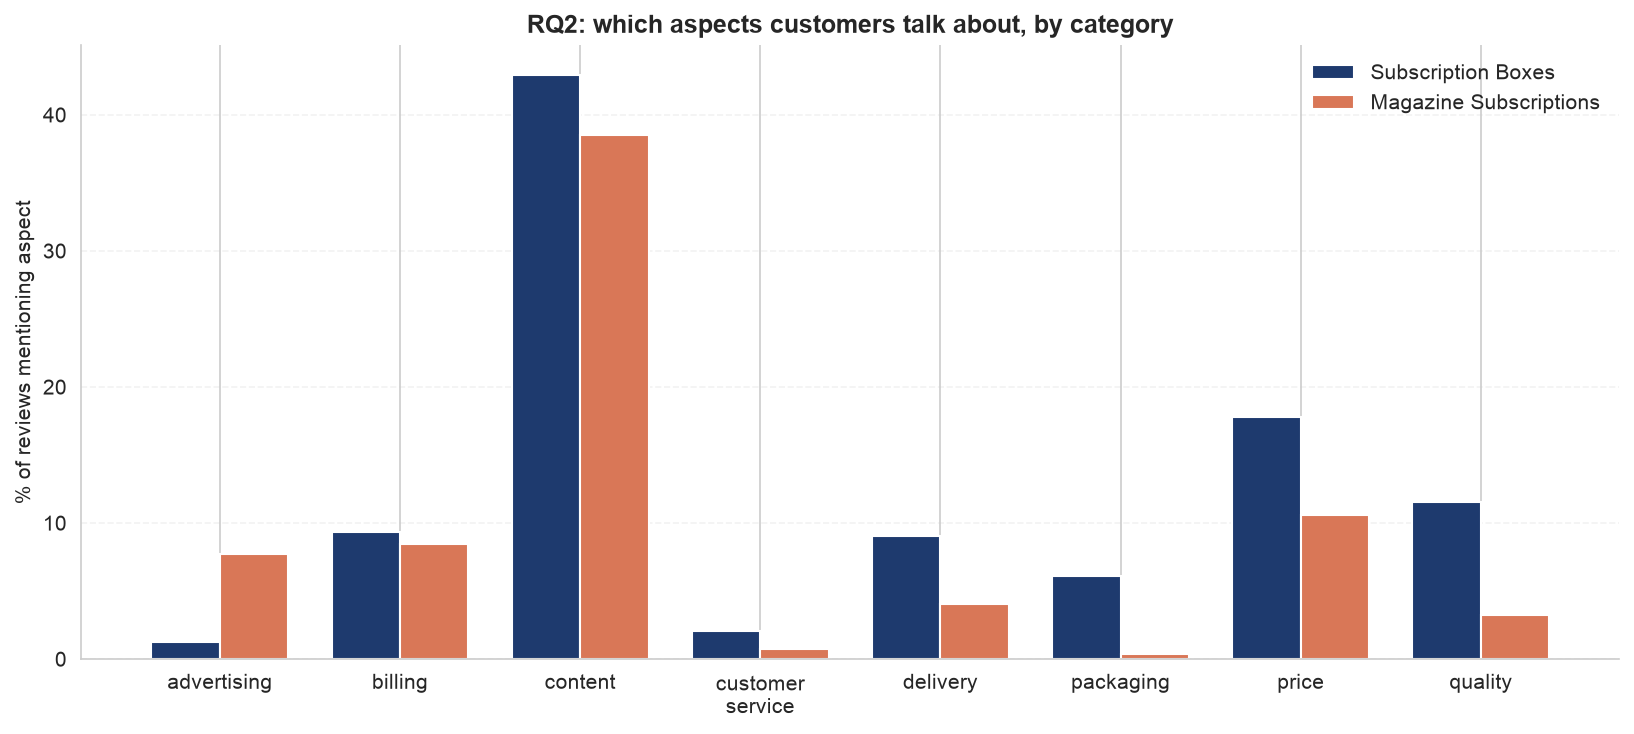
\includegraphics[width=0.9\textwidth]{rq2_mention_rate.png}
\caption{Share of reviews mentioning each aspect, by category. \emph{Content}
drives magazines; \emph{packaging} drives subscription boxes.}
\label{fig:rq2mention}
\end{figure}

\subsection{Aspect sentiment}
The radar and bar views (Figures \ref{fig:rq2radar}, \ref{fig:rq2sent}) and Table
\ref{tab:rq2} agree on one striking pattern: in \emph{both} categories,
\emph{billing} has by far the lowest mean sentiment (compound $\approx
0.17$--$0.18$) and the highest negative share ($21\%$ for magazines, $28\%$ for
boxes), while \emph{content} and \emph{price} are the most positive (compound
$\approx 0.34$--$0.38$). The sentiment composition per aspect (Figure
\ref{fig:rq2sent}) shows the same: billing carries the largest red (negative)
band.

\begin{figure}[H]
\centering
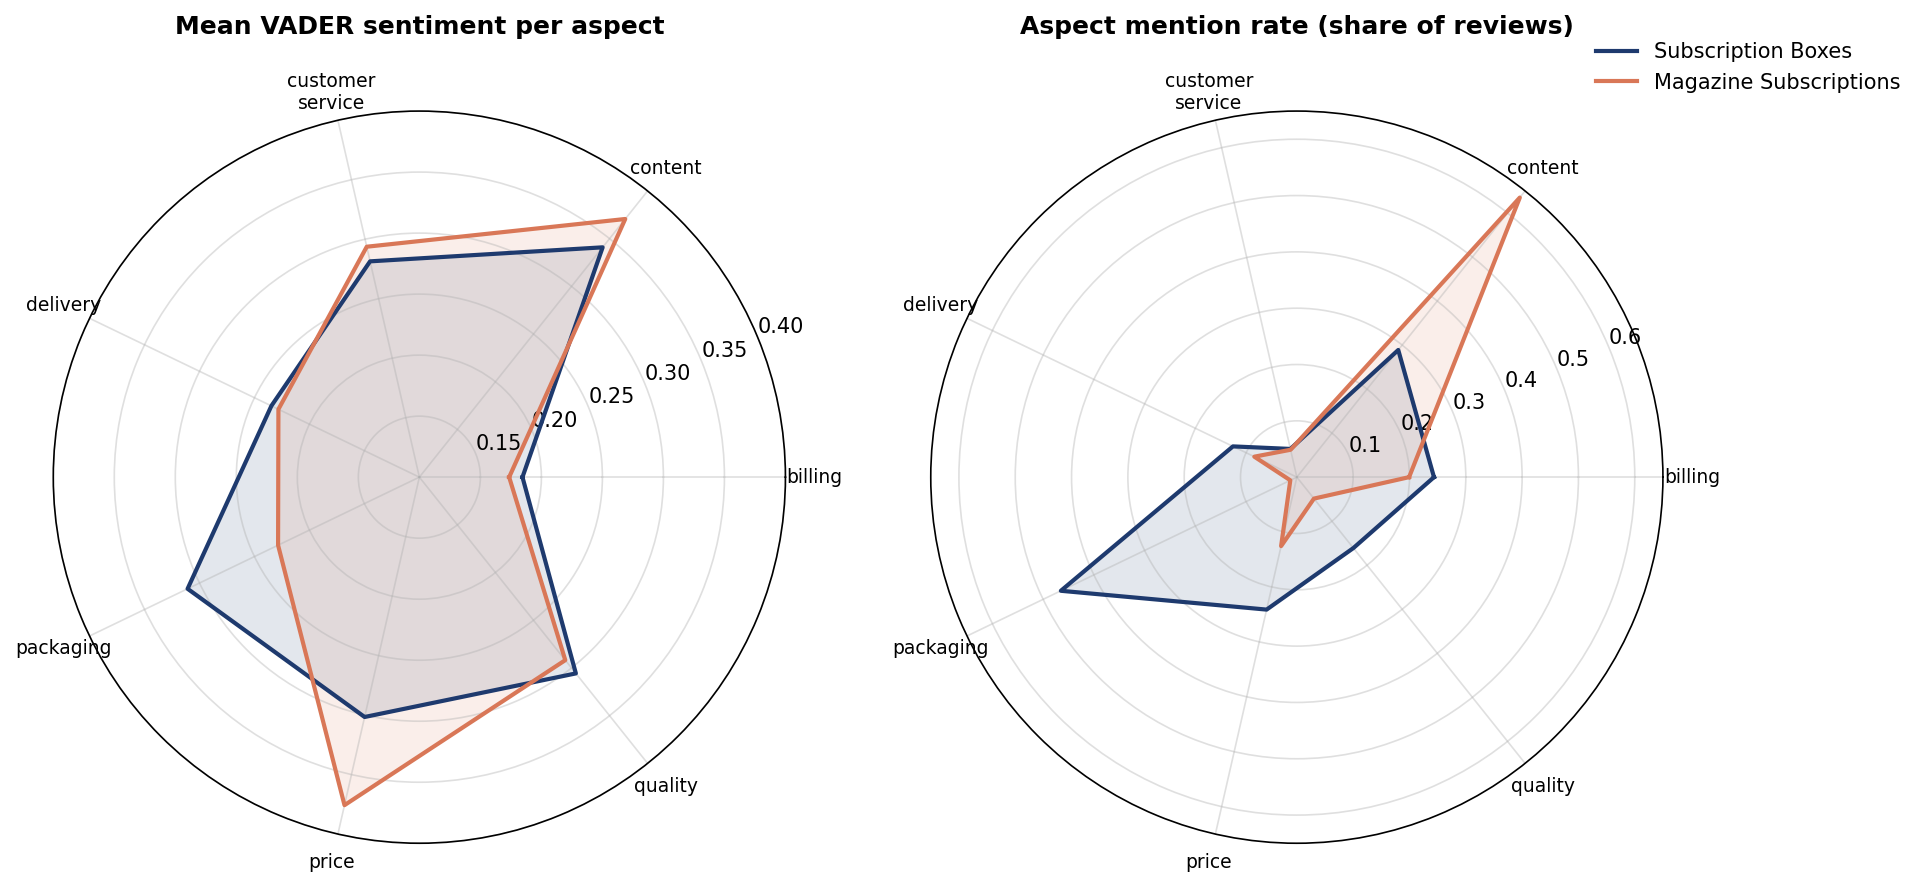
\includegraphics[width=\textwidth]{rq2_aspect_radar.png}
\caption{Aspect profiles as radar charts. Left: mean VADER sentiment --- both
polygons collapse inward at \emph{billing}. Right: mention rate --- the
categories' different shapes (content vs.\ packaging).}
\label{fig:rq2radar}
\end{figure}

\begin{table}[H]
\centering
\caption{Per-aspect mention rate, mean VADER compound and negative share, by
category. Lowest sentiment per category in \textbf{bold}.}
\label{tab:rq2}
\setlength{\tabcolsep}{5pt}
\begin{tabular}{l rrr rrr}
\toprule
& \multicolumn{3}{c}{Subscription Boxes} & \multicolumn{3}{c}{Magazine Subscriptions}\\
\cmidrule(lr){2-4}\cmidrule(lr){5-7}
Aspect & Mention\,\% & Mean & Neg\,\% & Mention\,\% & Mean & Neg\,\% \\
\midrule
billing          & 24.4 & \textbf{0.185} & 27.8 & 19.9 & \textbf{0.174} & 21.0 \\
content          & 28.9 & 0.341 & 13.5 & 63.5 & 0.371 & 8.7 \\
customer service & 5.1  & 0.281 & 20.4 & 5.0  & 0.294 & 21.9 \\
delivery         & 12.6 & 0.235 & 19.4 & 8.4  & 0.228 & 14.2 \\
packaging        & 46.5 & 0.311 & 14.8 & 1.3  & 0.229 & 19.2 \\
price            & 24.1 & 0.302 & 20.1 & 12.6 & 0.376 & 12.9 \\
quality          & 16.1 & 0.306 & 15.0 & 4.9  & 0.292 & 13.1 \\
\bottomrule
\end{tabular}
\end{table}

\begin{figure}[H]
\centering
\begin{subfigure}{0.49\textwidth}
  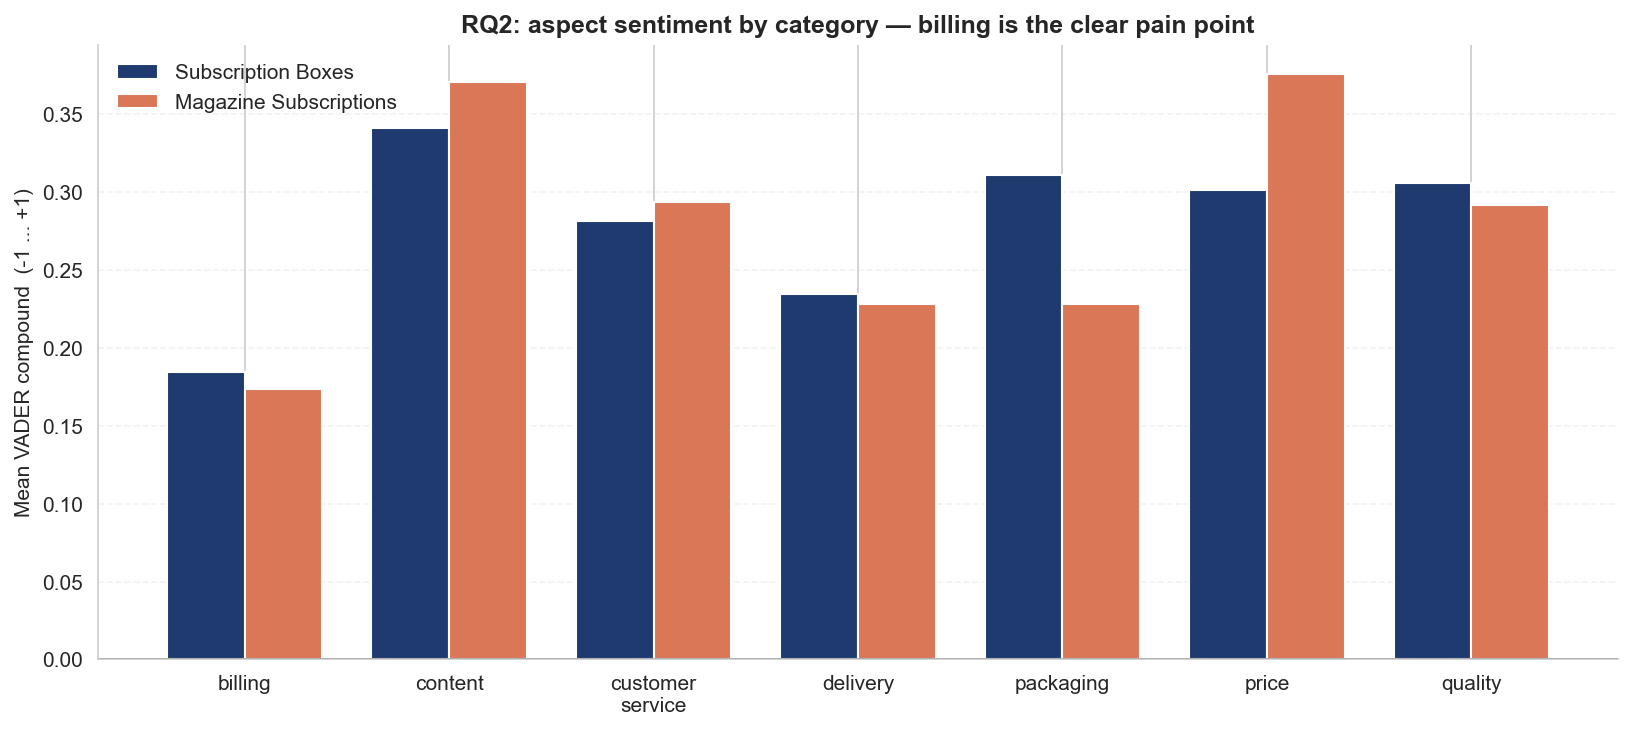
\includegraphics[width=\linewidth]{rq2_aspect_sentiment.png}
  \caption{Mean sentiment per aspect.}
\end{subfigure}\hfill
\begin{subfigure}{0.49\textwidth}
  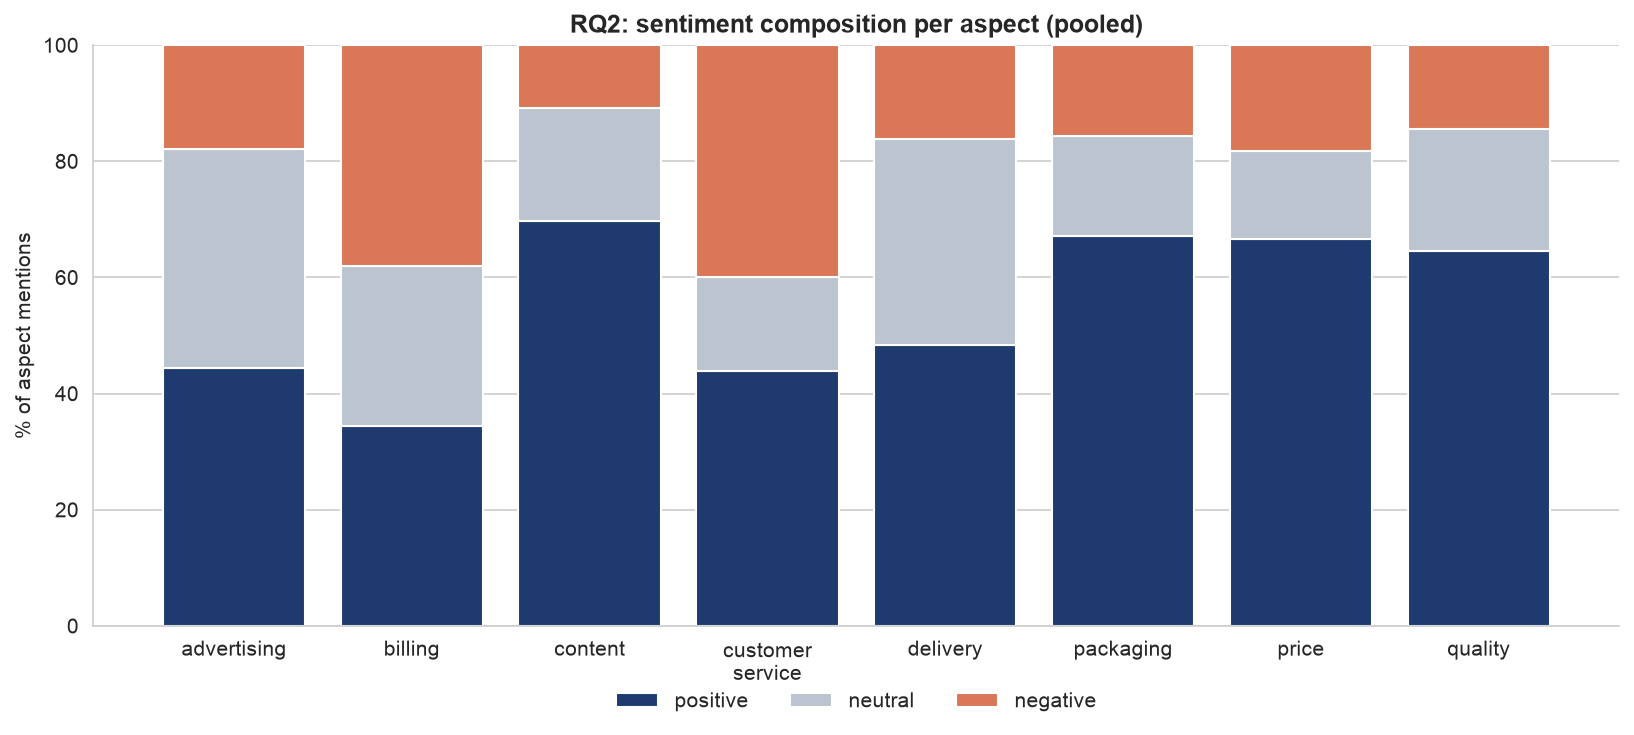
\includegraphics[width=\linewidth]{rq2_sentiment_composition.png}
  \caption{Sentiment composition (pooled).}
\end{subfigure}
\caption{Aspect sentiment as bars and as positive/neutral/negative composition.
Billing is the most negative aspect on both views.}
\label{fig:rq2sent}
\end{figure}

\subsection{Noun-phrase view}
The most frequent noun phrases (Figure \ref{fig:rq2np}) independently validate
the lexicon: \emph{the box, the toys, the products, the price, the items} for
boxes and \emph{this magazine, the articles, subscription} for magazines all map
onto the predefined aspects. (One data artefact: a stray \texttt{br} token for
magazines, a remnant of \texttt{<br>} HTML tags in the raw text, which the
noun-phrase view uses unmodified; it does not affect the keyword/VADER pipeline.)

\begin{figure}[H]
\centering
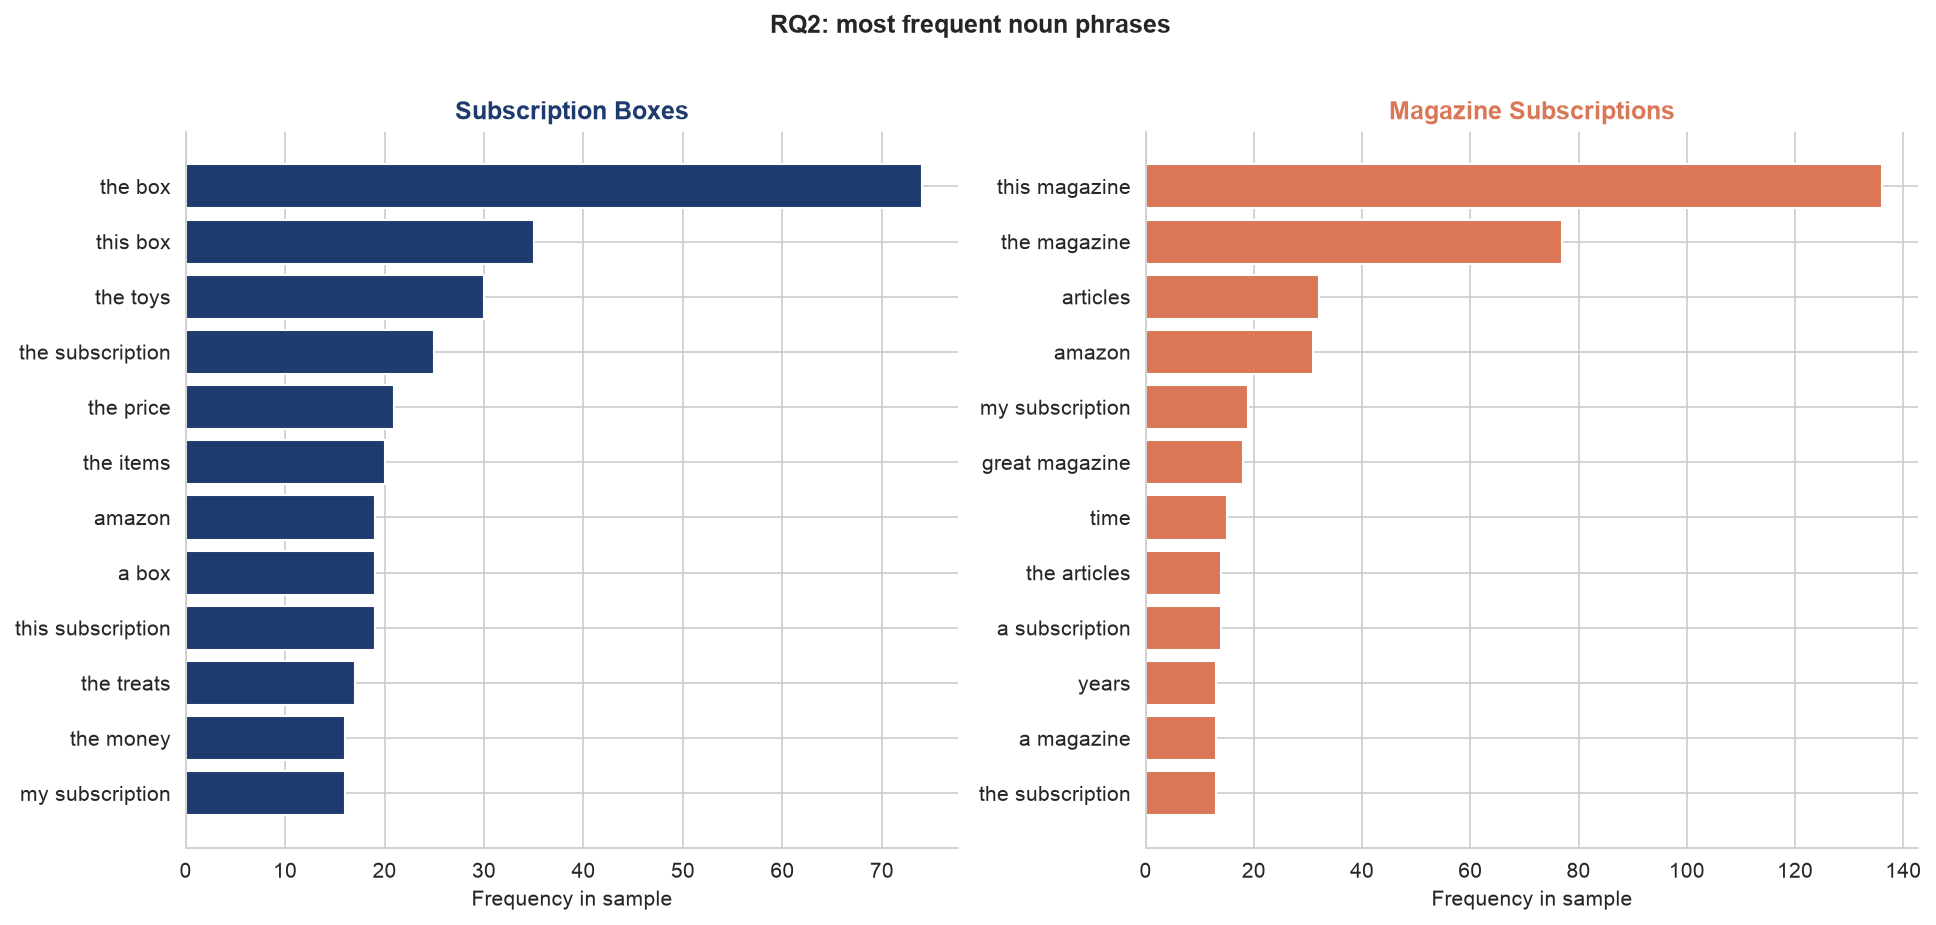
\includegraphics[width=\textwidth]{rq2_noun_phrases.png}
\caption{Most frequent noun phrases per category --- a data-driven cross-check of
the keyword aspect lexicon.}
\label{fig:rq2np}
\end{figure}

\subsection{Robustness: VADER versus the classifier}
\label{sec:rq2-robust}
On a test-set sample, VADER and the RQ1 classifier agree on $\approx\!75\%$ of
non-neutral aspect mentions (Table \ref{tab:agree}) --- close enough to confirm
VADER is not producing noise, divergent enough to matter. Importantly, VADER
labels about $22\%$ of mentions \emph{neutral}, a category the binary classifier
structurally cannot express. Combined with the out-of-distribution concern, this
justifies VADER as the primary sentence-level scorer and the classifier as a
sanity check only.

\begin{table}[H]
\centering
\caption{Agreement between VADER and the document classifier on non-neutral
aspect mentions (test sample).}
\label{tab:agree}
\begin{tabular}{lrr}
\toprule
Aspect & Agreement & $n$ \\
\midrule
content          & 0.803 & 639 \\
packaging        & 0.737 & 114 \\
quality          & 0.737 & 76 \\
price            & 0.730 & 137 \\
billing          & 0.690 & 203 \\
customer service & 0.679 & 56 \\
delivery         & 0.602 & 83 \\
\midrule
\textbf{Overall} & \textbf{$\approx$0.75} & 1{,}308 \\
\bottomrule
\end{tabular}
\end{table}

\subsection{Qualitative lexicon validation}
Because no gold aspect labels exist, we inspected a sample of aspect-assigned
sentences (Appendix \ref{app:val}). The keyword lexicon assigns aspects correctly
in the large majority of cases; the main failure mode is incidental keyword use
(e.g.\ ``value'' meaning worth-as-virtue rather than price). This, and the
single-score-per-sentence limitation, are discussed next.

% ============================ 7 DISCUSSION ==================================
\section{Discussion}
\label{sec:discussion}

\paragraph{Performance versus interpretability (Main RQ).}
On these high-dimensional, sparse TF-IDF features, the fully interpretable
Logistic Regression is the best model under both framings and is \emph{not}
outperformed by gradient boosting (binary macro-F1 $0.870$ vs.\ $0.834$). The
intuition is standard: linear models excel when the signal is largely additive
over many sparse lexical features, where tree ensembles gain little. The headline
finding for the Main RQ is therefore encouraging --- for this task, choosing the
transparent model costs essentially no accuracy, and it buys a model whose every
decision can be traced to specific words (Table \ref{tab:coef}).

\paragraph{Two methods, one conclusion.}
The most negative coefficient of the supervised classifier (\emph{cancel}) and
the most negative aspect of the unsupervised VADER pipeline (\emph{billing})
identify the \emph{same} business problem from two independent directions. For
subscription products, dissatisfaction is concentrated not in product quality but
in the billing and cancellation experience --- a directly actionable insight.

\paragraph{Label noise and the neutral ceiling.}
The error analysis showed that star ratings and text sentiment genuinely
disagree for a non-trivial set of reviews, and the ternary results showed the
3-star class cannot be reliably separated. Both point to the same truth: the
star rating is a noisy, coarse label, and the hardest reviews are the genuinely
mixed ones --- exactly where aspect-level analysis adds value over a single
document label.

\paragraph{Business implications.}
A practitioner can deploy the balanced Logistic Regression as a transparent
polarity monitor, and the lexicon+VADER layer as an aspect dashboard that flags
\emph{which} facet drives sentiment. For both subscription categories, the first
intervention the data recommends is fixing billing/cancellation friction.

% ============================ 8 LIMITATIONS =================================
\section{Limitations and Future Work}
\label{sec:limitations}

\begin{itemize}[leftmargin=1.4em]
  \item \textbf{Sentence-level attribution} cannot separate two aspects that
  co-occur in one sentence with mixed sentiment (``great content \dots but
  overpriced''): both inherit the sentence's single VADER score. Clause-level
  splitting on coordinating conjunctions is the natural refinement.
  \item \textbf{Lexicon and scorer} are hand-built and English-only, and VADER is
  general-purpose rather than domain-tuned; a domain-adapted lexicon would
  improve precision.
  \item \textbf{No gold aspect labels} exist, so RQ2 is validated only against a
  second method and qualitative inspection, not ground truth. A small annotated
  set (SemEval-style, \citealp{pontiki2014semeval}) would enable proper scoring.
  \item \textbf{Star ratings as labels} are noisy, as the error analysis showed,
  placing a ceiling on supervised accuracy.
  \item \textbf{Category scope:} Subscription Boxes has only 641 distinct items,
  so its aspect frequencies can be influenced by a few popular boxes.
  \item \textbf{Neural contrast:} a transparent linear model was the goal here; a
  controlled comparison against a Sentence-BERT classifier
  \citep{reimers2019sentencebert} would quantify the interpretability--accuracy
  frontier more precisely.
\end{itemize}

% ============================ 9 CONCLUSION ==================================
\section{Conclusion}
\label{sec:conclusion}

We built a fully classical, reproducible NLP pipeline that turns 87{,}713 Amazon
subscription reviews into structured opinion data. For document-level polarity,
class imbalance --- not model choice --- is the dominant evaluation concern: a
$69\%$-accurate baseline identifies no negatives, and only after explicit
rebalancing do the models recall the minority class well, with an interpretable
balanced Logistic Regression the strongest ($0.87$ macro-F1) and as good as
gradient boosting. For aspect-based sentiment, a sentence-level lexicon+VADER
pipeline shows that \emph{what} customers discuss is category-specific (content
vs.\ packaging) while \emph{what frustrates} them is shared and concentrated in
\emph{billing}. That the interpretable classifier's strongest negative word is
\emph{cancel} --- the same billing signal --- is the study's central result:
on this task, interpretability is essentially free, and the transparent model
hands the business a directly actionable diagnosis.

% ============================ REFERENCES ====================================
\bibliographystyle{plainnat}
\bibliography{references}

% ============================ APPENDIX ======================================
\appendix
\section{Additional material}
\label{app:val}
The repository accompanying this paper contains the full result tables and
figures, including per-class precision/recall/F1, the complete top-noun-phrase
lists per category, and the sampled aspect-assigned sentences used for the
qualitative lexicon validation (\texttt{results/tables/}). All notebooks
(\texttt{01\_eda} through \texttt{05\_paper\_figures}) reproduce every figure and
table from the raw data.

\vfill
\begin{center}\textbf{Declaration of Originality}\end{center}
\noindent
I declare that I have authored this paper independently, that I have not used
other than the declared sources / resources, and that I have explicitly marked
all material which has been quoted either literally or by content from the used
sources.
\vspace{1.5cm}

\noindent
\theplace, \today \hfill \rule{6cm}{0.4pt}\\
\phantom{\theplace, \today} \hfill \theauthor

\end{document}
